\noindent The scripts below belong to a sprite named Cat: \\

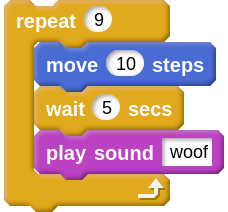
\includegraphics[scale=.3]{q1_script0.png} \hspace{1cm}
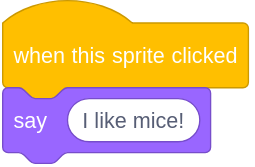
\includegraphics[scale=.3]{q1_script1.png} \hspace{1cm}
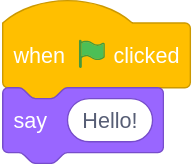
\includegraphics[scale=.3]{q1_script2.png} \hspace{1cm}
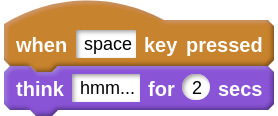
\includegraphics[scale=.3]{q1_script3.png} \hspace{1cm} \\

\noindent 1. \textbf{Circle}: What should you do to make Cat say "Hello!"?
\renewcommand{\theenumi}{\Alph{enumi}}
\begin{enumerate}
\item Press the space key
\item Click the green flag
\item Press the down arrow
\item Click the sprite
\end{enumerate}

\noindent \dotfill \\

\noindent 2. \textbf{Circle} the Say block that will be run \underline{last}.  \\
\begin{center}
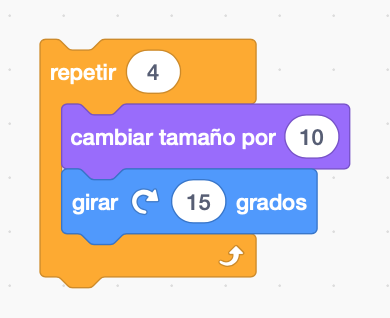
\includegraphics[scale=.3]{q2_script0.png}
\end{center}

\noindent \dotfill \\